\documentclass[tikz,border=10pt]{standalone}
% No TikZ libraries needed for this figure.
\begin{document}
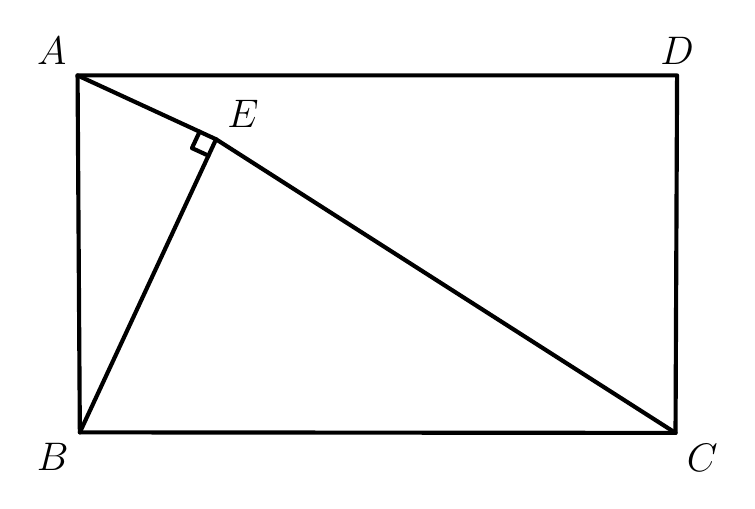
\begin{tikzpicture}[line width=1.5pt, line join=round, line cap=round]
  % Named coordinates: scale s = 0.019324 cm/px, origin at rectangle centre (244,182.5) px
  \coordinate (A) at (-3.807,  2.270);
  \coordinate (B) at (-3.778, -2.263);
  \coordinate (C) at ( 3.787, -2.270);
  \coordinate (D) at ( 3.807,  2.270);
  \coordinate (E) at (-2.048,  1.459);

  % Rectangle ABCD (solid)
  \draw (A) -- (B) -- (C) -- (D) -- cycle;

  % Segments AE and EC (bend at E), and BE
  \draw (A) -- (E) -- (C);
  \draw (B) -- (E);

  % Right-angle marker at E (one mark, on the EA/EB wedge)
  \draw (-2.257,1.555) -- (-2.354,1.347) -- (-2.145,1.251);

  % Labels
  \node[above left]  at (A) {\fontsize{15.5}{18.6}\selectfont $A$};
  \node[above]       at (D) {\fontsize{15.5}{18.6}\selectfont $D$};
  \node[below left]  at (B) {\fontsize{15.5}{18.6}\selectfont $B$};
  \node[below right] at (C) {\fontsize{15.5}{18.6}\selectfont $C$};
  \node[above right] at (E) {\fontsize{15.5}{18.6}\selectfont $E$};
\end{tikzpicture}
\end{document}